\documentclass{beamer}
%
% Choose how your presentation looks.
%
% For more themes, color themes and font themes, see:
% http://deic.uab.es/~iblanes/beamer_gallery/index_by_theme.html
%
\mode<presentation>
{
  \usetheme{Marburg}      % or try Darmstadt, Madrid, Warsaw, ...
  \usecolortheme{default} % or try albatross, beaver, crane, ...
  \usefonttheme{default}  % or try serif, structurebold, ...
  \setbeamertemplate{navigation symbols}{}
  \setbeamertemplate{caption}[numbered]
} 

\usepackage[english]{babel}
\usepackage[utf8]{inputenc}
\usepackage[T1]{fontenc}
\usepackage{natbib}

\title{Detecting Toxic Content from Social Media using LLMs}
\author[Naman Chhibbar \\ Meka Nani]{Naman Chhibbar, Meka Nani}
\institute{Indian Institute of Technology Hyderabad}
\date{27 September 2024}

\begin{document}

  \begin{frame}
    \titlepage
    \begin{center}
        \textit{\scriptsize Warning: This presentation contains sensitive content}
    \end{center}
  \end{frame}

\section{Introduction}

\begin{frame}{Introduction}

\begin{itemize}

    \item Toxicity in natural language refers to expressing hate or stereotypes towards an individual or a group of people using language.

    \item In general, toxic content can be categorized into:
    \begin{itemize}
        \item \textbf{Derogation:} Insulting or demeaning a group of individuals.
        \item \textbf{Animosity:} Subtly abusing a group (without using explicit language).
        \item \textbf{Threatening:} Expression of intent to harm, supporting harmful act, or encouraging inflicting harm on an individual or a group.
        \item \textbf{Supporting toxicity:} Encouraging, justifying, or glorifying hateful acts.
        \item \textbf{Dehumanizing:} Treating an individual or a group as "less human" (for example, insects, animals, etc.).
    \end{itemize}

\end{itemize}

\end{frame}

\section{Problem Statement}

Given some social media content (in the form of natural language), we want to predict whether it is toxic; this makes this task a binary classification problem.
Formally speaking, given a natural language input $x = (w_1, w_2, \dots, w_n)$, we need to predict if $x$ is toxic.

\section{Datasets}

\begin{frame}{Datasets}

  \begin{itemize}
  
    \item ToxicGen \citep{hartvigsen2022toxigen}
    \begin{itemize}
      \item Created by prompting an LLM to produce toxic and benign texts.
      \item Texts do not contain explicit language and target minority groups.
      \item Example: Muslims deserve to die.
    \end{itemize}
    
    \item SBIC (Social Bias Inference Corpus) \citep{zhang2024efficient}
    \begin{itemize}
      \item Texts contain stereotypes and offensiveness towards an individual or a group of people.
      \item Example: Women candidates are less qualified.
    \end{itemize}

    \item DHate \citep{vidgen2020learning}
    \begin{itemize}
      \item Details about this dataset are not revealed.
      \item From manual analysis, this dataset seems to be comprised of hate of minorities.
      \item Example: I always feel unsafe when surrounded by Arabs.
    \end{itemize}

  \end{itemize}
    
\end{frame}

\section{Challenges}

\begin{frame}{Challenges}

% \begin{itemize}

%     \item Performance relies heavily on the quality of prompts
%     \item Deploying LLMs for toxic content detection can incur both high run-time costs and high latency 
%     \item \textbf{Existing works}-Bootstrapping and Distilling LLM's
%     \begin{itemize}
%         \item Decision-Tree-of-Thought
%         \item Fine-tune a suitable student LM with a smaller model size
%     \end{itemize}
%     \begin{figure}
%         \centering
%         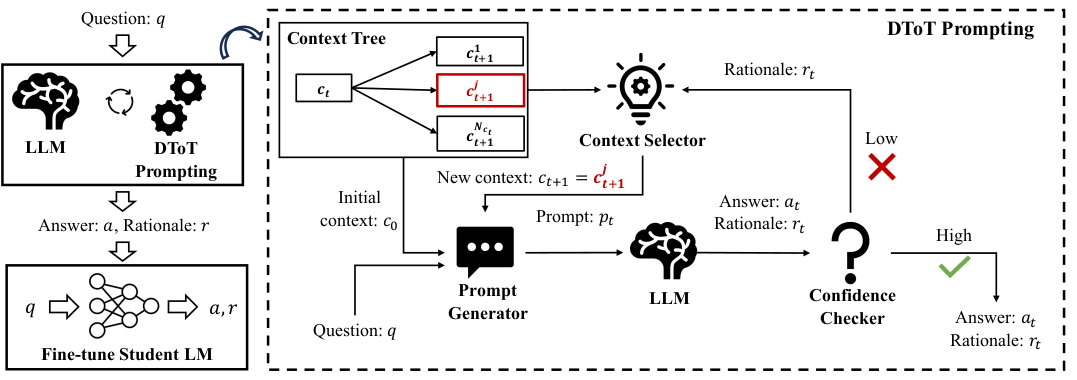
\includegraphics[width=1\linewidth]{images/BD_LLM.png}
%         \caption{Illustration of BD-LLM}
%         \label{fig:1}
%     \end{figure}

% \end{itemize}

\begin{itemize}

    \item A major challenge in detecting toxicity is that toxicity is relative.
    \item Some may think that some content is toxic, while others may not.
    \item This happens due to different perceptions of people.
    \item In addition, the datasets being used are also biased.
    \item For example:
    \begin{itemize}
        \item "I'm going to kill Amy" is labelled as not toxic in the DHate dataset, whereas it falls in the "Threatening" category.
        \item "A dude with money can only impress a broke bitch" is labelled as not toxic in the SBIC dataset, whereas many may think it is (due to vulgarity).
    \end{itemize}

\end{itemize}

\begin{itemize}
    \item 
\end{itemize}

\end{frame}

\section{Related Works}

\begin{frame}{Related Works}
    \begin{itemize}
        \item 
    \end{itemize}
\end{frame}

\section{Proposed Methods}


\begin{frame}{Good-old BERT}

  \begin{itemize}
    \item BERT has long been used to classify texts.
    \item Even with the challenges posed by toxic content, we wish to experiment with the classic method of using BERT with a classifier head.
  \end{itemize}

\end{frame}


\begin{frame}{Classification with KNNs}

  \begin{itemize}
    \item This approach maintains a vector database of toxic examples.
    \item When we get a new input, we use the vector database to extract k-nearest-neighbours toxic examples.
    \item We then use these examples for k-shot prompting.
    \item For classification, we can either use a transformer with a classifier head or an API call to an LLM (for example, GPT) to get a "yes" or "no" output.
  \end{itemize}
    
\end{frame}


\begin{frame}{Classification with KNNs}

  \begin{figure}
    \centering
    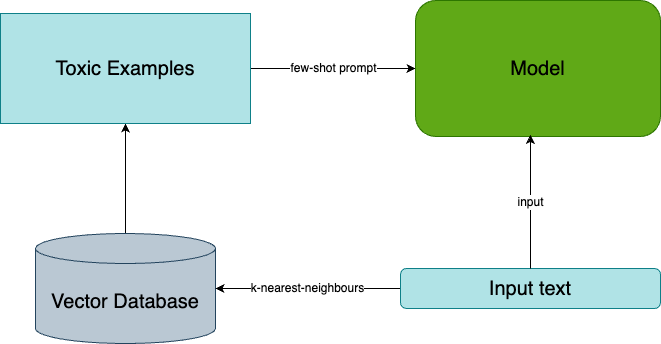
\includegraphics[width=0.8\linewidth]{images/architecture.png}
    \caption{Architecture}
  \end{figure}

\end{frame}

\section{Questions}

\begin{frame}
  \centering

  \huge Thank you for listening!
  \vskip 1cm
  \large Feel free to ask questions

\end{frame}


% \begin{frame}{References}
%     \bibliography{anthology}
% \end{frame}

\end{document}
